\documentclass[1p]{elsarticle_modified}
%\bibliographystyle{elsarticle-num}

%\usepackage[colorlinks]{hyperref}
%\usepackage{abbrmath_seonhwa} %\Abb, \Ascr, \Acal ,\Abf, \Afrak
\usepackage{amsfonts}
\usepackage{amssymb}
\usepackage{amsmath}
\usepackage{amsthm}
\usepackage{scalefnt}
\usepackage{amsbsy}
\usepackage{kotex}
\usepackage{caption}
\usepackage{subfig}
\usepackage{color}
\usepackage{graphicx}
\usepackage{xcolor} %% white, black, red, green, blue, cyan, magenta, yellow
\usepackage{float}
\usepackage{setspace}
\usepackage{hyperref}

\usepackage{tikz}
\usetikzlibrary{arrows}

\usepackage{multirow}
\usepackage{array} % fixed length table
\usepackage{hhline}

%%%%%%%%%%%%%%%%%%%%%
\makeatletter
\renewcommand*\env@matrix[1][\arraystretch]{%
	\edef\arraystretch{#1}%
	\hskip -\arraycolsep
	\let\@ifnextchar\new@ifnextchar
	\array{*\c@MaxMatrixCols c}}
\makeatother %https://tex.stackexchange.com/questions/14071/how-can-i-increase-the-line-spacing-in-a-matrix
%%%%%%%%%%%%%%%

\usepackage[normalem]{ulem}

\newcommand{\msout}[1]{\ifmmode\text{\sout{\ensuremath{#1}}}\else\sout{#1}\fi}
%SOURCE: \msout is \stkout macro in https://tex.stackexchange.com/questions/20609/strikeout-in-math-mode

\newcommand{\cancel}[1]{
	\ifmmode
	{\color{red}\msout{#1}}
	\else
	{\color{red}\sout{#1}}
	\fi
}

\newcommand{\add}[1]{
	{\color{blue}\uwave{#1}}
}

\newcommand{\replace}[2]{
	\ifmmode
	{\color{red}\msout{#1}}{\color{blue}\uwave{#2}}
	\else
	{\color{red}\sout{#1}}{\color{blue}\uwave{#2}}
	\fi
}

\newcommand{\Sol}{\mathcal{S}} %segment
\newcommand{\D}{D} %diagram
\newcommand{\A}{\mathcal{A}} %arc


%%%%%%%%%%%%%%%%%%%%%%%%%%%%%5 test

\def\sl{\operatorname{\textup{SL}}(2,\Cbb)}
\def\psl{\operatorname{\textup{PSL}}(2,\Cbb)}
\def\quan{\mkern 1mu \triangleright \mkern 1mu}

\theoremstyle{definition}
\newtheorem{thm}{Theorem}[section]
\newtheorem{prop}[thm]{Proposition}
\newtheorem{lem}[thm]{Lemma}
\newtheorem{ques}[thm]{Question}
\newtheorem{cor}[thm]{Corollary}
\newtheorem{defn}[thm]{Definition}
\newtheorem{exam}[thm]{Example}
\newtheorem{rmk}[thm]{Remark}
\newtheorem{alg}[thm]{Algorithm}

\newcommand{\I}{\sqrt{-1}}
\begin{document}

%\begin{frontmatter}
%
%\title{Boundary parabolic representations of knots up to 8 crossings}
%
%%% Group authors per affiliation:
%\author{Yunhi Cho} 
%\address{Department of Mathematics, University of Seoul, Seoul, Korea}
%\ead{yhcho@uos.ac.kr}
%
%
%\author{Seonhwa Kim} %\fnref{s_kim}}
%\address{Center for Geometry and Physics, Institute for Basic Science, Pohang, 37673, Korea}
%\ead{ryeona17@ibs.re.kr}
%
%\author{Hyuk Kim}
%\address{Department of Mathematical Sciences, Seoul National University, Seoul 08826, Korea}
%\ead{hyukkim@snu.ac.kr}
%
%\author{Seokbeom Yoon}
%\address{Department of Mathematical Sciences, Seoul National University, Seoul, 08826,  Korea}
%\ead{sbyoon15@snu.ac.kr}
%
%\begin{abstract}
%We find all boundary parabolic representation of knots up to 8 crossings.
%
%\end{abstract}
%\begin{keyword}
%    \MSC[2010] 57M25 
%\end{keyword}
%
%\end{frontmatter}

%\linenumbers
%\tableofcontents
%
\newcommand\colored[1]{\textcolor{white}{\rule[-0.35ex]{0.8em}{1.4ex}}\kern-0.8em\color{red} #1}%
%\newcommand\colored[1]{\textcolor{white}{ #1}\kern-2.17ex	\textcolor{white}{ #1}\kern-1.81ex	\textcolor{white}{ #1}\kern-2.15ex\color{red}#1	}

{\Large $\underline{11n_{54}~(K11n_{54})}$}

\setlength{\tabcolsep}{10pt}
\renewcommand{\arraystretch}{1.6}
\vspace{1cm}\begin{tabular}{m{100pt}>{\centering\arraybackslash}m{274pt}}
\multirow{5}{120pt}{
	\centering
	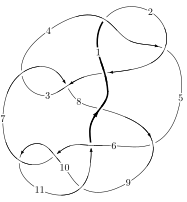
\includegraphics[width=112pt]{../../../GIT/diagram.site/Diagrams/png/670_11n_54.png}\\
\ \ \ A knot diagram\footnotemark}&
\allowdisplaybreaks
\textbf{Linearized knot diagam} \\
\cline{2-2}
 &
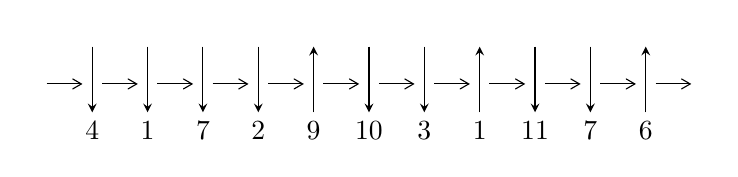
\begin{tikzpicture}[x=20pt, y=17pt]
	% nodes
	\node (C0) at (0, 0) {};
	\node (C1) at (1, 0) {};
	\node (C1U) at (1, +1) {};
	\node (C1D) at (1, -1) {4};

	\node (C2) at (2, 0) {};
	\node (C2U) at (2, +1) {};
	\node (C2D) at (2, -1) {1};

	\node (C3) at (3, 0) {};
	\node (C3U) at (3, +1) {};
	\node (C3D) at (3, -1) {7};

	\node (C4) at (4, 0) {};
	\node (C4U) at (4, +1) {};
	\node (C4D) at (4, -1) {2};

	\node (C5) at (5, 0) {};
	\node (C5U) at (5, +1) {};
	\node (C5D) at (5, -1) {9};

	\node (C6) at (6, 0) {};
	\node (C6U) at (6, +1) {};
	\node (C6D) at (6, -1) {10};

	\node (C7) at (7, 0) {};
	\node (C7U) at (7, +1) {};
	\node (C7D) at (7, -1) {3};

	\node (C8) at (8, 0) {};
	\node (C8U) at (8, +1) {};
	\node (C8D) at (8, -1) {1};

	\node (C9) at (9, 0) {};
	\node (C9U) at (9, +1) {};
	\node (C9D) at (9, -1) {11};

	\node (C10) at (10, 0) {};
	\node (C10U) at (10, +1) {};
	\node (C10D) at (10, -1) {7};

	\node (C11) at (11, 0) {};
	\node (C11U) at (11, +1) {};
	\node (C11D) at (11, -1) {6};
	\node (C12) at (12, 0) {};

	% arrows
	\draw[->,>={angle 60}]
	(C0) edge (C1) (C1) edge (C2) (C2) edge (C3) (C3) edge (C4) (C4) edge (C5) (C5) edge (C6) (C6) edge (C7) (C7) edge (C8) (C8) edge (C9) (C9) edge (C10) (C10) edge (C11) (C11) edge (C12) ;	\draw[->,>=stealth]
	(C1U) edge (C1D) (C2U) edge (C2D) (C3U) edge (C3D) (C4U) edge (C4D) (C5D) edge (C5U) (C6U) edge (C6D) (C7U) edge (C7D) (C8D) edge (C8U) (C9U) edge (C9D) (C10U) edge (C10D) (C11D) edge (C11U) ;
	\end{tikzpicture} \\
\hhline{~~} \\& 
\textbf{Solving Sequence} \\ \cline{2-2} 
 &
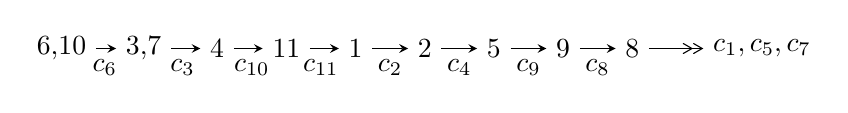
\begin{tikzpicture}[x=25pt, y=7pt]
	% node
	\node (A0) at (-1/8, 0) {6,10};
	\node (A1) at (17/16, 0) {3,7};
	\node (A2) at (17/8, 0) {4};
	\node (A3) at (25/8, 0) {11};
	\node (A4) at (33/8, 0) {1};
	\node (A5) at (41/8, 0) {2};
	\node (A6) at (49/8, 0) {5};
	\node (A7) at (57/8, 0) {9};
	\node (A8) at (65/8, 0) {8};
	\node (C1) at (1/2, -1) {$c_{6}$};
	\node (C2) at (13/8, -1) {$c_{3}$};
	\node (C3) at (21/8, -1) {$c_{10}$};
	\node (C4) at (29/8, -1) {$c_{11}$};
	\node (C5) at (37/8, -1) {$c_{2}$};
	\node (C6) at (45/8, -1) {$c_{4}$};
	\node (C7) at (53/8, -1) {$c_{9}$};
	\node (C8) at (61/8, -1) {$c_{8}$};
	\node (A9) at (10, 0) {$c_{1},c_{5},c_{7}$};

	% edge
	\draw[->,>=stealth]	
	(A0) edge (A1) (A1) edge (A2) (A2) edge (A3) (A3) edge (A4) (A4) edge (A5) (A5) edge (A6) (A6) edge (A7) (A7) edge (A8) ;
	\draw[->>,>={angle 60}]	
	(A8) edge (A9);
\end{tikzpicture} \\ 

\end{tabular} \\

\footnotetext{
The image of knot diagram is generated by the software ``\textbf{Draw programme}" developed by Andrew Bartholomew(\url{http://www.layer8.co.uk/maths/draw/index.htm\#Running-draw}), where we modified some parts for our purpose(\url{https://github.com/CATsTAILs/LinksPainter}).
}\phantom \\ \newline 
\centering \textbf{Ideals for irreducible components\footnotemark of $X_{\text{par}}$} 
 
\begin{align*}
I^u_{1}&=\langle 
- u^{25}+u^{24}+\cdots+b- u,\;- u^{25}+u^{24}+\cdots+a+2,\;u^{27}-2 u^{26}+\cdots+4 u-1\rangle \\
I^u_{2}&=\langle 
- u^3+b+u+1,\;- u^4- u^3+u^2+a+u,\;u^6+u^5- u^4-2 u^3+u+1\rangle \\
\\
\end{align*}
\raggedright * 2 irreducible components of $\dim_{\mathbb{C}}=0$, with total 33 representations.\\
\footnotetext{All coefficients of polynomials are rational numbers. But the coefficients are sometimes approximated in decimal forms when there is not enough margin.}
\newpage
\renewcommand{\arraystretch}{1}
\centering \section*{I. $I^u_{1}= \langle - u^{25}+u^{24}+\cdots+b- u,\;- u^{25}+u^{24}+\cdots+a+2,\;u^{27}-2 u^{26}+\cdots+4 u-1 \rangle$}
\flushleft \textbf{(i) Arc colorings}\\
\begin{tabular}{m{7pt} m{180pt} m{7pt} m{180pt} }
\flushright $a_{6}=$&$\begin{pmatrix}1\\0\end{pmatrix}$ \\
\flushright $a_{10}=$&$\begin{pmatrix}0\\u\end{pmatrix}$ \\
\flushright $a_{3}=$&$\begin{pmatrix}u^{25}- u^{24}+\cdots+3 u^2-2\\u^{25}- u^{24}+\cdots+u^2+u\end{pmatrix}$ \\
\flushright $a_{7}=$&$\begin{pmatrix}1\\u^2\end{pmatrix}$ \\
\flushright $a_{4}=$&$\begin{pmatrix}u^{26}- u^{25}+\cdots-5 u-1\\- u^{26}+u^{25}+\cdots-2 u^2+2 u\end{pmatrix}$ \\
\flushright $a_{11}=$&$\begin{pmatrix}- u\\- u^3+u\end{pmatrix}$ \\
\flushright $a_{1}=$&$\begin{pmatrix}- u^3\\- u^3+u\end{pmatrix}$ \\
\flushright $a_{2}=$&$\begin{pmatrix}- u^{24}+u^{23}+\cdots-3 u-1\\- u^{26}+u^{25}+\cdots-5 u^3+2 u\end{pmatrix}$ \\
\flushright $a_{5}=$&$\begin{pmatrix}- u^8+u^6- u^4-1\\- u^{10}+2 u^8-3 u^6+2 u^4- u^2\end{pmatrix}$ \\
\flushright $a_{9}=$&$\begin{pmatrix}u^3\\u^5- u^3+u\end{pmatrix}$ \\
\flushright $a_{8}=$&$\begin{pmatrix}- u^{11}+2 u^9-2 u^7+u^3\\- u^{11}+3 u^9-4 u^7+3 u^5- u^3+u\end{pmatrix}$\\ \flushright $a_{8}=$&$\begin{pmatrix}- u^{11}+2 u^9-2 u^7+u^3\\- u^{11}+3 u^9-4 u^7+3 u^5- u^3+u\end{pmatrix}$\\&\end{tabular}
\flushleft \textbf{(ii) Obstruction class $= -1$}\\~\\
\flushleft \textbf{(iii) Cusp Shapes $= -4 u^{26}+6 u^{25}+20 u^{24}-39 u^{23}-47 u^{22}+126 u^{21}+51 u^{20}-259 u^{19}+17 u^{18}+366 u^{17}-150 u^{16}-376 u^{15}+266 u^{14}+292 u^{13}-287 u^{12}-189 u^{11}+231 u^{10}+112 u^9-162 u^8-61 u^7+97 u^6+36 u^5-47 u^4-23 u^3+17 u^2+12 u-14$}\\~\\
\newpage\renewcommand{\arraystretch}{1}
\flushleft \textbf{(iv) u-Polynomials at the component}\newline \\
\begin{tabular}{m{50pt}|m{274pt}}
Crossings & \hspace{64pt}u-Polynomials at each crossing \\
\hline $$\begin{aligned}c_{1},c_{4}\end{aligned}$$&$\begin{aligned}
&u^{27}-7 u^{26}+\cdots-5 u+1
\end{aligned}$\\
\hline $$\begin{aligned}c_{2}\end{aligned}$$&$\begin{aligned}
&u^{27}+3 u^{26}+\cdots+5 u+1
\end{aligned}$\\
\hline $$\begin{aligned}c_{3},c_{7}\end{aligned}$$&$\begin{aligned}
&u^{27}+u^{26}+\cdots+128 u+64
\end{aligned}$\\
\hline $$\begin{aligned}c_{5}\end{aligned}$$&$\begin{aligned}
&u^{27}-2 u^{26}+\cdots+2 u+1
\end{aligned}$\\
\hline $$\begin{aligned}c_{6},c_{10}\end{aligned}$$&$\begin{aligned}
&u^{27}+2 u^{26}+\cdots+4 u+1
\end{aligned}$\\
\hline $$\begin{aligned}c_{8}\end{aligned}$$&$\begin{aligned}
&u^{27}+8 u^{26}+\cdots+16990 u+565
\end{aligned}$\\
\hline $$\begin{aligned}c_{9}\end{aligned}$$&$\begin{aligned}
&u^{27}+12 u^{26}+\cdots+12 u+1
\end{aligned}$\\
\hline $$\begin{aligned}c_{11}\end{aligned}$$&$\begin{aligned}
&u^{27}+6 u^{26}+\cdots+48 u+5
\end{aligned}$\\
\hline
\end{tabular}\\~\\
\newpage\renewcommand{\arraystretch}{1}
\flushleft \textbf{(v) Riley Polynomials at the component}\newline \\
\begin{tabular}{m{50pt}|m{274pt}}
Crossings & \hspace{64pt}Riley Polynomials at each crossing \\
\hline $$\begin{aligned}c_{1},c_{4}\end{aligned}$$&$\begin{aligned}
&y^{27}-3 y^{26}+\cdots+5 y-1
\end{aligned}$\\
\hline $$\begin{aligned}c_{2}\end{aligned}$$&$\begin{aligned}
&y^{27}+49 y^{26}+\cdots-23 y-1
\end{aligned}$\\
\hline $$\begin{aligned}c_{3},c_{7}\end{aligned}$$&$\begin{aligned}
&y^{27}+39 y^{26}+\cdots-28672 y-4096
\end{aligned}$\\
\hline $$\begin{aligned}c_{5}\end{aligned}$$&$\begin{aligned}
&y^{27}-36 y^{26}+\cdots+12 y-1
\end{aligned}$\\
\hline $$\begin{aligned}c_{6},c_{10}\end{aligned}$$&$\begin{aligned}
&y^{27}-12 y^{26}+\cdots+12 y-1
\end{aligned}$\\
\hline $$\begin{aligned}c_{8}\end{aligned}$$&$\begin{aligned}
&y^{27}-72 y^{26}+\cdots+171458760 y-319225
\end{aligned}$\\
\hline $$\begin{aligned}c_{9}\end{aligned}$$&$\begin{aligned}
&y^{27}+8 y^{26}+\cdots+32 y-1
\end{aligned}$\\
\hline $$\begin{aligned}c_{11}\end{aligned}$$&$\begin{aligned}
&y^{27}-4 y^{26}+\cdots+504 y-25
\end{aligned}$\\
\hline
\end{tabular}\\~\\
\newpage\flushleft \textbf{(vi) Complex Volumes and Cusp Shapes}
$$\begin{array}{c|c|c}  
\text{Solutions to }I^u_{1}& \I (\text{vol} + \sqrt{-1}CS) & \text{Cusp shape}\\
 \hline 
\begin{aligned}
u &= -0.917142 + 0.407659 I \\
a &= \phantom{-}1.20846 + 2.04717 I \\
b &= \phantom{-}2.09938 + 1.19019 I\end{aligned}
 & -2.84916 + 1.60658 I & -4.88146 - 5.04321 I \\ \hline\begin{aligned}
u &= -0.917142 - 0.407659 I \\
a &= \phantom{-}1.20846 - 2.04717 I \\
b &= \phantom{-}2.09938 - 1.19019 I\end{aligned}
 & -2.84916 - 1.60658 I & -4.88146 + 5.04321 I \\ \hline\begin{aligned}
u &= \phantom{-}0.526875 + 0.831344 I \\
a &= \phantom{-}0.11316 - 2.41248 I \\
b &= \phantom{-}1.82470 - 0.93091 I\end{aligned}
 & \phantom{-}12.17430 - 2.19817 I & -0.63423 + 2.08830 I \\ \hline\begin{aligned}
u &= \phantom{-}0.526875 - 0.831344 I \\
a &= \phantom{-}0.11316 + 2.41248 I \\
b &= \phantom{-}1.82470 + 0.93091 I\end{aligned}
 & \phantom{-}12.17430 + 2.19817 I & -0.63423 - 2.08830 I \\ \hline\begin{aligned}
u &= \phantom{-}0.467388 + 0.843376 I \\
a &= -0.08288 + 2.25887 I \\
b &= -2.19783 + 0.76965 I\end{aligned}
 & \phantom{-}11.82210 + 5.91141 I & -1.03607 - 2.33228 I \\ \hline\begin{aligned}
u &= \phantom{-}0.467388 - 0.843376 I \\
a &= -0.08288 - 2.25887 I \\
b &= -2.19783 - 0.76965 I\end{aligned}
 & \phantom{-}11.82210 - 5.91141 I & -1.03607 + 2.33228 I \\ \hline\begin{aligned}
u &= \phantom{-}0.971756 + 0.498250 I \\
a &= \phantom{-}0.462169 - 0.060454 I \\
b &= -0.404355 + 0.874051 I\end{aligned}
 & -2.13464 - 3.70052 I & -7.14700 + 4.32876 I \\ \hline\begin{aligned}
u &= \phantom{-}0.971756 - 0.498250 I \\
a &= \phantom{-}0.462169 + 0.060454 I \\
b &= -0.404355 - 0.874051 I\end{aligned}
 & -2.13464 + 3.70052 I & -7.14700 - 4.32876 I \\ \hline\begin{aligned}
u &= \phantom{-}1.059940 + 0.286714 I \\
a &= -0.219785 - 0.584186 I \\
b &= \phantom{-}0.225820 - 0.093826 I\end{aligned}
 & -2.30226 - 0.55935 I & -5.41913 - 0.15707 I \\ \hline\begin{aligned}
u &= \phantom{-}1.059940 - 0.286714 I \\
a &= -0.219785 + 0.584186 I \\
b &= \phantom{-}0.225820 + 0.093826 I\end{aligned}
 & -2.30226 + 0.55935 I & -5.41913 + 0.15707 I\\
 \hline 
 \end{array}$$\newpage$$\begin{array}{c|c|c}  
\text{Solutions to }I^u_{1}& \I (\text{vol} + \sqrt{-1}CS) & \text{Cusp shape}\\
 \hline 
\begin{aligned}
u &= -0.580852 + 0.656113 I \\
a &= -0.834314 - 0.778452 I \\
b &= -1.197700 - 0.124667 I\end{aligned}
 & \phantom{-}2.76848 + 0.13713 I & \phantom{-}0.773547 - 0.780119 I \\ \hline\begin{aligned}
u &= -0.580852 - 0.656113 I \\
a &= -0.834314 + 0.778452 I \\
b &= -1.197700 + 0.124667 I\end{aligned}
 & \phantom{-}2.76848 - 0.13713 I & \phantom{-}0.773547 + 0.780119 I \\ \hline\begin{aligned}
u &= -1.001280 + 0.594918 I \\
a &= -0.59412 - 1.46994 I \\
b &= -1.21967 - 0.98587 I\end{aligned}
 & \phantom{-}1.53114 + 4.74698 I & -2.05877 - 5.37624 I \\ \hline\begin{aligned}
u &= -1.001280 - 0.594918 I \\
a &= -0.59412 + 1.46994 I \\
b &= -1.21967 + 0.98587 I\end{aligned}
 & \phantom{-}1.53114 - 4.74698 I & -2.05877 + 5.37624 I \\ \hline\begin{aligned}
u &= -1.175710 + 0.039463 I \\
a &= -0.392154 - 0.491529 I \\
b &= -0.267337 + 1.188470 I\end{aligned}
 & \phantom{-}5.98407 - 3.79755 I & -6.46791 + 2.18250 I \\ \hline\begin{aligned}
u &= -1.175710 - 0.039463 I \\
a &= -0.392154 + 0.491529 I \\
b &= -0.267337 - 1.188470 I\end{aligned}
 & \phantom{-}5.98407 + 3.79755 I & -6.46791 - 2.18250 I \\ \hline\begin{aligned}
u &= -1.103060 + 0.538696 I \\
a &= \phantom{-}1.181940 - 0.254407 I \\
b &= \phantom{-}0.857869 - 0.770675 I\end{aligned}
 & -0.58075 + 6.65503 I & -3.43691 - 7.46005 I \\ \hline\begin{aligned}
u &= -1.103060 - 0.538696 I \\
a &= \phantom{-}1.181940 + 0.254407 I \\
b &= \phantom{-}0.857869 + 0.770675 I\end{aligned}
 & -0.58075 - 6.65503 I & -3.43691 + 7.46005 I \\ \hline\begin{aligned}
u &= -0.326760 + 0.690469 I \\
a &= -0.462660 + 0.572854 I \\
b &= \phantom{-}0.218748 + 0.864330 I\end{aligned}
 & \phantom{-}1.66847 - 1.93992 I & \phantom{-}0.12713 + 2.72762 I \\ \hline\begin{aligned}
u &= -0.326760 - 0.690469 I \\
a &= -0.462660 - 0.572854 I \\
b &= \phantom{-}0.218748 - 0.864330 I\end{aligned}
 & \phantom{-}1.66847 + 1.93992 I & \phantom{-}0.12713 - 2.72762 I\\
 \hline 
 \end{array}$$\newpage$$\begin{array}{c|c|c}  
\text{Solutions to }I^u_{1}& \I (\text{vol} + \sqrt{-1}CS) & \text{Cusp shape}\\
 \hline 
\begin{aligned}
u &= \phantom{-}0.698871 + 0.307602 I \\
a &= -0.894710 + 0.463414 I \\
b &= \phantom{-}0.205039 - 0.148466 I\end{aligned}
 & -1.077410 - 0.093546 I & -6.21440 - 0.06252 I \\ \hline\begin{aligned}
u &= \phantom{-}0.698871 - 0.307602 I \\
a &= -0.894710 - 0.463414 I \\
b &= \phantom{-}0.205039 + 0.148466 I\end{aligned}
 & -1.077410 + 0.093546 I & -6.21440 + 0.06252 I \\ \hline\begin{aligned}
u &= \phantom{-}1.074550 + 0.661713 I \\
a &= \phantom{-}2.00442 - 1.14909 I \\
b &= \phantom{-}3.21245 - 0.01349 I\end{aligned}
 & \phantom{-}10.52730 - 3.36992 I & -2.71394 + 2.50695 I \\ \hline\begin{aligned}
u &= \phantom{-}1.074550 - 0.661713 I \\
a &= \phantom{-}2.00442 + 1.14909 I \\
b &= \phantom{-}3.21245 + 0.01349 I\end{aligned}
 & \phantom{-}10.52730 + 3.36992 I & -2.71394 - 2.50695 I \\ \hline\begin{aligned}
u &= \phantom{-}1.106510 + 0.642553 I \\
a &= -2.19489 + 1.59992 I \\
b &= -3.52700 + 0.08432 I\end{aligned}
 & \phantom{-}9.8976 - 11.4401 I & -3.60368 + 6.65783 I \\ \hline\begin{aligned}
u &= \phantom{-}1.106510 - 0.642553 I \\
a &= -2.19489 - 1.59992 I \\
b &= -3.52700 - 0.08432 I\end{aligned}
 & \phantom{-}9.8976 + 11.4401 I & -3.60368 - 6.65783 I \\ \hline\begin{aligned}
u &= \phantom{-}0.397840\phantom{ +0.000000I} \\
a &= -1.58927\phantom{ +0.000000I} \\
b &= \phantom{-}0.339752\phantom{ +0.000000I}\end{aligned}
 & -1.09734\phantom{ +0.000000I} & -8.57440\phantom{ +0.000000I}\\
 \hline 
 \end{array}$$\newpage\newpage\renewcommand{\arraystretch}{1}
\centering \section*{II. $I^u_{2}= \langle - u^3+b+u+1,\;- u^4- u^3+u^2+a+u,\;u^6+u^5- u^4-2 u^3+u+1 \rangle$}
\flushleft \textbf{(i) Arc colorings}\\
\begin{tabular}{m{7pt} m{180pt} m{7pt} m{180pt} }
\flushright $a_{6}=$&$\begin{pmatrix}1\\0\end{pmatrix}$ \\
\flushright $a_{10}=$&$\begin{pmatrix}0\\u\end{pmatrix}$ \\
\flushright $a_{3}=$&$\begin{pmatrix}u^4+u^3- u^2- u\\u^3- u-1\end{pmatrix}$ \\
\flushright $a_{7}=$&$\begin{pmatrix}1\\u^2\end{pmatrix}$ \\
\flushright $a_{4}=$&$\begin{pmatrix}u^4+u^3- u^2- u\\u^3- u-1\end{pmatrix}$ \\
\flushright $a_{11}=$&$\begin{pmatrix}- u\\- u^3+u\end{pmatrix}$ \\
\flushright $a_{1}=$&$\begin{pmatrix}- u^3\\- u^3+u\end{pmatrix}$ \\
\flushright $a_{2}=$&$\begin{pmatrix}u^4- u^2- u\\-1\end{pmatrix}$ \\
\flushright $a_{5}=$&$\begin{pmatrix}u^3\\u^3- u\end{pmatrix}$ \\
\flushright $a_{9}=$&$\begin{pmatrix}u^3\\u^5- u^3+u\end{pmatrix}$ \\
\flushright $a_{8}=$&$\begin{pmatrix}1\\u^2\end{pmatrix}$\\ \flushright $a_{8}=$&$\begin{pmatrix}1\\u^2\end{pmatrix}$\\&\end{tabular}
\flushleft \textbf{(ii) Obstruction class $= 1$}\\~\\
\flushleft \textbf{(iii) Cusp Shapes $= 4 u^4-5 u^2-5 u-5$}\\~\\
\newpage\renewcommand{\arraystretch}{1}
\flushleft \textbf{(iv) u-Polynomials at the component}\newline \\
\begin{tabular}{m{50pt}|m{274pt}}
Crossings & \hspace{64pt}u-Polynomials at each crossing \\
\hline $$\begin{aligned}c_{1}\end{aligned}$$&$\begin{aligned}
&(u-1)^6
\end{aligned}$\\
\hline $$\begin{aligned}c_{2},c_{4}\end{aligned}$$&$\begin{aligned}
&(u+1)^6
\end{aligned}$\\
\hline $$\begin{aligned}c_{3},c_{7}\end{aligned}$$&$\begin{aligned}
&u^6
\end{aligned}$\\
\hline $$\begin{aligned}c_{5},c_{8},c_{10}\end{aligned}$$&$\begin{aligned}
&u^6- u^5- u^4+2 u^3- u+1
\end{aligned}$\\
\hline $$\begin{aligned}c_{6}\end{aligned}$$&$\begin{aligned}
&u^6+u^5- u^4-2 u^3+u+1
\end{aligned}$\\
\hline $$\begin{aligned}c_{9},c_{11}\end{aligned}$$&$\begin{aligned}
&u^6-3 u^5+5 u^4-4 u^3+2 u^2- u+1
\end{aligned}$\\
\hline
\end{tabular}\\~\\
\newpage\renewcommand{\arraystretch}{1}
\flushleft \textbf{(v) Riley Polynomials at the component}\newline \\
\begin{tabular}{m{50pt}|m{274pt}}
Crossings & \hspace{64pt}Riley Polynomials at each crossing \\
\hline $$\begin{aligned}c_{1},c_{2},c_{4}\end{aligned}$$&$\begin{aligned}
&(y-1)^6
\end{aligned}$\\
\hline $$\begin{aligned}c_{3},c_{7}\end{aligned}$$&$\begin{aligned}
&y^6
\end{aligned}$\\
\hline $$\begin{aligned}c_{5},c_{6},c_{8}\\c_{10}\end{aligned}$$&$\begin{aligned}
&y^6-3 y^5+5 y^4-4 y^3+2 y^2- y+1
\end{aligned}$\\
\hline $$\begin{aligned}c_{9},c_{11}\end{aligned}$$&$\begin{aligned}
&y^6+y^5+5 y^4+6 y^2+3 y+1
\end{aligned}$\\
\hline
\end{tabular}\\~\\
\newpage\flushleft \textbf{(vi) Complex Volumes and Cusp Shapes}
$$\begin{array}{c|c|c}  
\text{Solutions to }I^u_{2}& \I (\text{vol} + \sqrt{-1}CS) & \text{Cusp shape}\\
 \hline 
\begin{aligned}
u &= \phantom{-}1.002190 + 0.295542 I \\
a &= -0.685196 + 1.063260 I \\
b &= -1.258210 + 0.569162 I\end{aligned}
 & -3.53554 - 0.92430 I & -12.63596 - 0.09369 I \\ \hline\begin{aligned}
u &= \phantom{-}1.002190 - 0.295542 I \\
a &= -0.685196 - 1.063260 I \\
b &= -1.258210 - 0.569162 I\end{aligned}
 & -3.53554 + 0.92430 I & -12.63596 + 0.09369 I \\ \hline\begin{aligned}
u &= -0.428243 + 0.664531 I \\
a &= \phantom{-}0.917982 + 0.270708 I \\
b &= -0.082955 - 0.592379 I\end{aligned}
 & \phantom{-}0.245672 - 0.924305 I & -2.59683 + 0.69886 I \\ \hline\begin{aligned}
u &= -0.428243 - 0.664531 I \\
a &= \phantom{-}0.917982 - 0.270708 I \\
b &= -0.082955 + 0.592379 I\end{aligned}
 & \phantom{-}0.245672 + 0.924305 I & -2.59683 - 0.69886 I \\ \hline\begin{aligned}
u &= -1.073950 + 0.558752 I \\
a &= -0.732786 + 0.381252 I \\
b &= -0.158836 + 1.200140 I\end{aligned}
 & -1.64493 + 5.69302 I & -6.76721 - 4.86918 I \\ \hline\begin{aligned}
u &= -1.073950 - 0.558752 I \\
a &= -0.732786 - 0.381252 I \\
b &= -0.158836 - 1.200140 I\end{aligned}
 & -1.64493 - 5.69302 I & -6.76721 + 4.86918 I\\
 \hline 
 \end{array}$$\newpage
\newpage\renewcommand{\arraystretch}{1}
\centering \section*{ III. u-Polynomials}
\begin{tabular}{m{50pt}|m{274pt}}
Crossings & \hspace{64pt}u-Polynomials at each crossing \\
\hline $$\begin{aligned}c_{1}\end{aligned}$$&$\begin{aligned}
&((u-1)^6)(u^{27}-7 u^{26}+\cdots-5 u+1)
\end{aligned}$\\
\hline $$\begin{aligned}c_{2}\end{aligned}$$&$\begin{aligned}
&((u+1)^6)(u^{27}+3 u^{26}+\cdots+5 u+1)
\end{aligned}$\\
\hline $$\begin{aligned}c_{3},c_{7}\end{aligned}$$&$\begin{aligned}
&u^6(u^{27}+u^{26}+\cdots+128 u+64)
\end{aligned}$\\
\hline $$\begin{aligned}c_{4}\end{aligned}$$&$\begin{aligned}
&((u+1)^6)(u^{27}-7 u^{26}+\cdots-5 u+1)
\end{aligned}$\\
\hline $$\begin{aligned}c_{5}\end{aligned}$$&$\begin{aligned}
&(u^6- u^5- u^4+2 u^3- u+1)(u^{27}-2 u^{26}+\cdots+2 u+1)
\end{aligned}$\\
\hline $$\begin{aligned}c_{6}\end{aligned}$$&$\begin{aligned}
&(u^6+u^5- u^4-2 u^3+u+1)(u^{27}+2 u^{26}+\cdots+4 u+1)
\end{aligned}$\\
\hline $$\begin{aligned}c_{8}\end{aligned}$$&$\begin{aligned}
&(u^6- u^5- u^4+2 u^3- u+1)(u^{27}+8 u^{26}+\cdots+16990 u+565)
\end{aligned}$\\
\hline $$\begin{aligned}c_{9}\end{aligned}$$&$\begin{aligned}
&(u^6-3 u^5+5 u^4-4 u^3+2 u^2- u+1)(u^{27}+12 u^{26}+\cdots+12 u+1)
\end{aligned}$\\
\hline $$\begin{aligned}c_{10}\end{aligned}$$&$\begin{aligned}
&(u^6- u^5- u^4+2 u^3- u+1)(u^{27}+2 u^{26}+\cdots+4 u+1)
\end{aligned}$\\
\hline $$\begin{aligned}c_{11}\end{aligned}$$&$\begin{aligned}
&(u^6-3 u^5+5 u^4-4 u^3+2 u^2- u+1)(u^{27}+6 u^{26}+\cdots+48 u+5)
\end{aligned}$\\
\hline
\end{tabular}\newpage\renewcommand{\arraystretch}{1}
\centering \section*{ IV. Riley Polynomials}
\begin{tabular}{m{50pt}|m{274pt}}
Crossings & \hspace{64pt}Riley Polynomials at each crossing \\
\hline $$\begin{aligned}c_{1},c_{4}\end{aligned}$$&$\begin{aligned}
&((y-1)^6)(y^{27}-3 y^{26}+\cdots+5 y-1)
\end{aligned}$\\
\hline $$\begin{aligned}c_{2}\end{aligned}$$&$\begin{aligned}
&((y-1)^6)(y^{27}+49 y^{26}+\cdots-23 y-1)
\end{aligned}$\\
\hline $$\begin{aligned}c_{3},c_{7}\end{aligned}$$&$\begin{aligned}
&y^6(y^{27}+39 y^{26}+\cdots-28672 y-4096)
\end{aligned}$\\
\hline $$\begin{aligned}c_{5}\end{aligned}$$&$\begin{aligned}
&(y^6-3 y^5+5 y^4-4 y^3+2 y^2- y+1)(y^{27}-36 y^{26}+\cdots+12 y-1)
\end{aligned}$\\
\hline $$\begin{aligned}c_{6},c_{10}\end{aligned}$$&$\begin{aligned}
&(y^6-3 y^5+5 y^4-4 y^3+2 y^2- y+1)(y^{27}-12 y^{26}+\cdots+12 y-1)
\end{aligned}$\\
\hline $$\begin{aligned}c_{8}\end{aligned}$$&$\begin{aligned}
&(y^6-3 y^5+5 y^4-4 y^3+2 y^2- y+1)\\
&\cdot(y^{27}-72 y^{26}+\cdots+171458760 y-319225)
\end{aligned}$\\
\hline $$\begin{aligned}c_{9}\end{aligned}$$&$\begin{aligned}
&(y^6+y^5+5 y^4+6 y^2+3 y+1)(y^{27}+8 y^{26}+\cdots+32 y-1)
\end{aligned}$\\
\hline $$\begin{aligned}c_{11}\end{aligned}$$&$\begin{aligned}
&(y^6+y^5+5 y^4+6 y^2+3 y+1)(y^{27}-4 y^{26}+\cdots+504 y-25)
\end{aligned}$\\
\hline
\end{tabular}
\vskip 2pc
\end{document}